%!TEX root = ../username.tex
\chapter{Interaction Systems}\label{interaction systems}


\section{Introduction to Unity}\label{Unity}
 
 Unity is a professional game engine that is used to create video games and virtual environments for a variety of platforms. Unity has two distinct advantages over other game development environments. The first is Unity's extremely user friendly visual workflow. Other game development tools are often overly complicated and require the user to set up their own integrated development environment, or IDE. Unity's visual editor is both sophisticated and extremely productive, allowing high quality games to be produced with relative ease and efficiency. The second advantage is Unity's wide array of cross-platform support. There are very few game engines that offer as many deployment targets, ranging from the PC, web and mobile to consoles. Unity also makes deploying to these platforms extremely simple. Compared to other game engines such as Unreal, CryEngine, or Game Maker, Unity stands in a fantastic middle ground in terms of the difficulty to learn and desired capabilities in engines. These comparisons and characteristics are brief examples of what makes Unity the engine of choice for many developers.
 
 \subsection{Unity's User Interface}
 
 Unity's user interface is split up into different tabs and sections as seen in Figure Blank
 
 %\ref{fig:UnityUI}. 
 
 The Project tab is used to view and access all the files in your project and the Console tab is available to view the output from your code. The Scene tab allows you to view the objects placed into the 3D scene and the Game tab lets you view the 3D scene as though the game is being played. The Hierarchy tab shows a list of all the objects in the scene and how they are nested in relation to each other. The Inspector tab displays information about the object selected and lets you change different components. The Toolbar provides scene navigation, including Move, Orbit, and Zoom functions. Unity's interface allows the user to easily create a 3D scene, however scripting is what brings a project to life. 
 
 %image insert
 
 \subsubsection{Scripting}
 
 \par Writing code in Unity is what controls your objects in the visual editor and makes the game interactive.  The game objects in Unity are built as a collection of components. This collection of components often include scripts, which refer to code files. Another nice aspect of Unity is code is not compiled and run as a separate executable, but instead executed within the Unity engine itself. Being able to test your game in a separate window without the inconvenience of having to create builds is very substantial. Unity supports both Javascript and C-sharp programming languages, although C-sharp is often preferred because it is strongly typed. When it comes time for writing scripts, picking an ideal IDE or text editor is important. Unity comes bundled with MonoDevelope, which is the IDE of choice because it is open source and offers cross-platform support for C-sharp. 

\subsection{Creating VR Through Unity}\label{creating VR through Unity}

\begin{figure}[h]
	\centering
	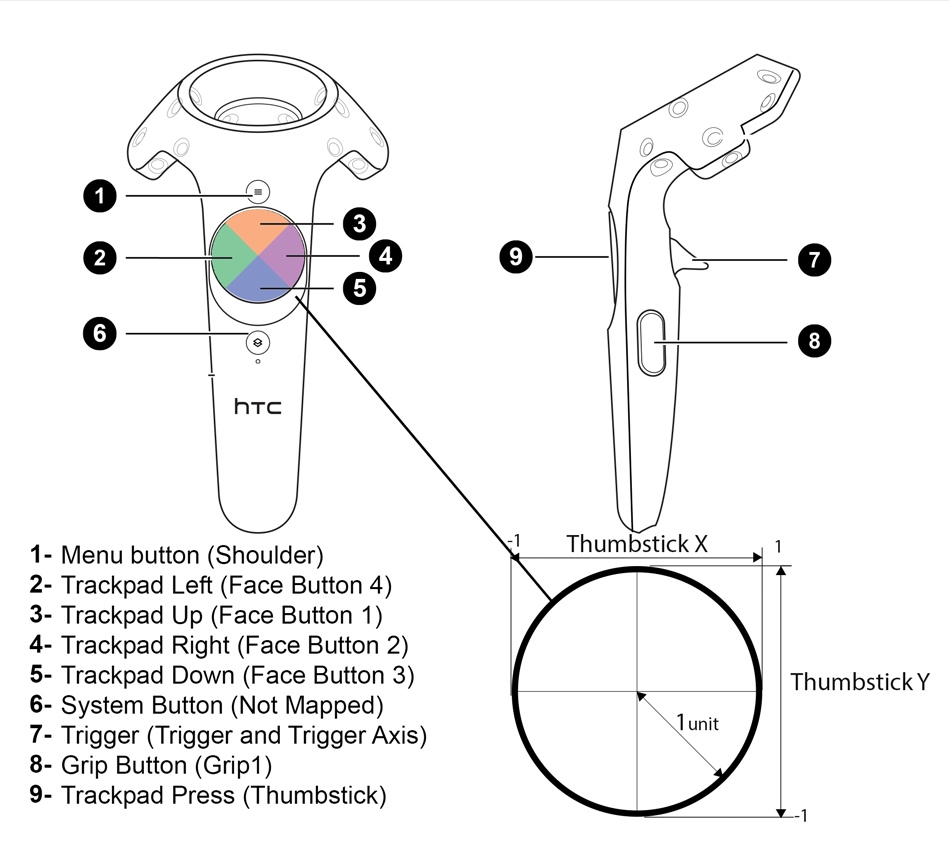
\includegraphics[width=.5\textwidth]{ViveControllers}
	\caption{Vive Controller Inputs \cite{ViveControllers}}
	\label{fig:ViveControllers}
\end{figure}

A distinct difference between virtual reality and an average game is the fact that when immersed in a virtual environment, quality is not just how good something looks, but how good something feels. Building an environment in Unity is one thing, but turning it into virtual reality involves a few extra steps. With a virtual reality application, different hardware is required, often with different types of input. With the HTC Vive, an effective user interface and realistic interaction systems must be implemented using the motion tracking capabilities and various input buttons on the Vive's controllers. Figure \ref{fig:ViveControllers} displays all the inputs that can be utilized by the controllers. 


\par A graphical user interface (GUI) is also essential for presenting information. A GUI refers to two-dimensional on screen graphics that overlay the main gameplay and present messages, gauges, or input controls such as menus buttons or sliders \cite{linowes}. In typical non VR games, a user interface is rendered in screen space, which statically rests somewhere on the screen as an overlay, such as a screen edge. In virtual reality, there are no screen edges, and the GUI must be rendered in what is called the World Space. Figure \ref{fig:GUI} shows a common approach taken by Oculus to display a main game menu. Although somewhat intrusive to the central scene, this style and placement for a GUI is easy to access a great alternative static main menu screen.

\begin{figure}[h]
	\centering
	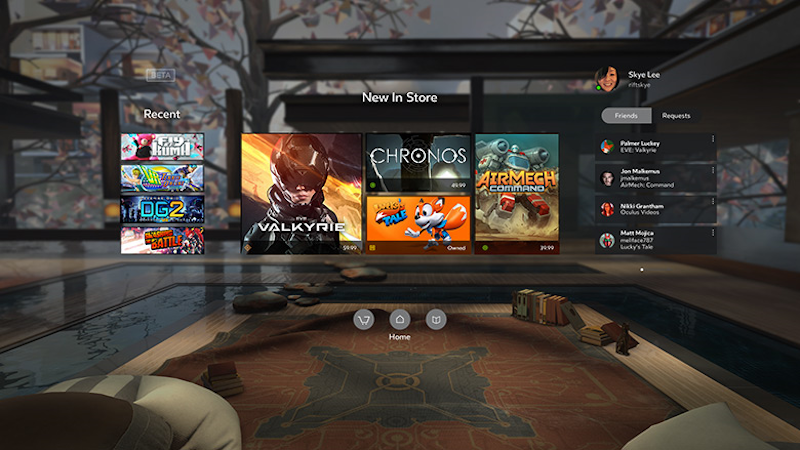
\includegraphics[width=.7\textwidth]{GUI}
	\caption{VR Game Menu - World Space \cite{GUI}}
	\label{fig:GUI}
\end{figure}




\subsection{VR Motion Sickness}

Despite the wonders of VR immersion, it is also known to cause feelings similar to motion sickness such as disorientation and nausea. VR motion sickness is a fairly substantial concern and is studied by many researchers, physiologists and technologists to find the underlying causes. We do know that lag caused by screen updates and synchronization problems when moving your head are a major contributing issue.
Given the potential impact rendering permanence, frames per second and latency have on a virtual reality application, optimizing implantation and content must be at the front of any developers mind \cite{gobbetti}. 
%Spatio-temporal realism, the ability to meet synchronization, lag, and accuracy constraints within low tolerates, has therefore become a required feature for virtual reality systems . 
Although these are the major issues corresponding to virtual reality motion sickness, there are a few others we should consider \cite{linowes}:

\begin{enumerate}
	\item Don't move too fast.
	\item Look forwards when moving through a scene.
	\item Avoid turning head too quickly.
	\item Use a third-person camera in certain settings.
	\item Provide visual cues to keep user grounded.
	\item Provide an option to recenter the view.
	\item Cut scenes break and transitions.
	\item Optimize rendering performance wherever possible.
\end{enumerate}

\section{Steam VR Plug-in}\label{steamVR}


\section{Naive System}\label{old}


\subsection{Allowances}\label{old _ allowances}


\subsection{Shortcomings}\label{old _ shortcomings}


\subsection{Improvements}\label{old _ improvements}


\section{Newtonian System}\label{new}


\subsection{Theory}\label{new _ theory}


\subsection{Allowances}\label{new _ allowances}


\subsection{Improvements}\label{new _ improvements}


